\documentclass{aastex62}

\usepackage{graphicx}
\usepackage{gensymb}
\usepackage{bm}
\usepackage{amsmath}

\newcommand{\Gus}[1]{\textcolor{red}{#1}}

\newcommand{\Msun}{\ensuremath{\text{M}_\odot}}
\newcommand{\pc}{\ensuremath{\text{pc}}}
\newcommand{\kpc}{\ensuremath{\text{kpc}}}
\newcommand{\Mpc}{\ensuremath{\text{Mpc}}}
\newcommand{\Myr}{\ensuremath{\text{Myr}}}
\newcommand{\Gyr}{\ensuremath{\text{Gyr}}}
\newcommand{\SFR}{\ensuremath{\text{SFR}}}

\newcommand{\MHz}{\ensuremath{\text{MHz}}}
\newcommand{\GHz}{\ensuremath{\text{GHz}}}

\newcommand{\CI}{\ensuremath{\text{C~\textsc{i}}}}
\newcommand{\CII}{\ensuremath{\text{C~\textsc{ii}}}}
\newcommand{\OIII}{\ensuremath{\text{O~\textsc{iii}}}}
\newcommand{\CO}{\ensuremath{\text{CO}}}

\newcommand{\abs}[1]{\left| #1 \right|}
\newcommand{\uth}{\textsuperscript{th}}
\newcommand{\n}{\text{n}}

\newcommand{\beq}{\begin{equation}}
\newcommand{\eeq}{\end{equation}}

\newcommand{\ps}[1]{\ensuremath{P_{#1,#1}}}
\newcommand{\xps}[2]{\ensuremath{P_{#1,#2}}}

\newcommand{\kmax}{\ensuremath{k_{\text{max}}}}

\newcommand{\mynu}[2]{\ensuremath{\nu_{#1,\text{#2}}}}
\newcommand{\denps}{\ensuremath{P_{\delta,\delta}}}
\newcommand{\pstot}[1]{\ensuremath{P_{#1,\text{tot}}}}
\newcommand{\Bsum}{\ensuremath{\tilde{B}}}

\newcommand{\kpar}{k_{\parallel}}
\newcommand{\kperp}{\bm{k}_{\perp}}
\newcommand{\apar}{\alpha_{\parallel}}
\newcommand{\aperp}{\alpha_{\perp}}

\newcommand{\E}[1]{\mathrm{E}[#1]}
\newcommand{\Var}[1]{\mathrm{Var}[#1]}
\newcommand{\Cov}[2]{\mathrm{Cov}[#1,#2]}
\newcommand{\avg}[1]{\ensuremath{\langle #1 \rangle}}
\newcommand{\SN}{\ensuremath{\text{S}/\text{N}}}

\newcommand{\bi}{\ensuremath{\avg{b_i}}}
\newcommand{\bj}{\ensuremath{\avg{b_j}}}
\newcommand{\Ii}{\ensuremath{\avg{I_i}}}
\newcommand{\Ij}{\ensuremath{\avg{I_j}}}

\newcommand{\penn}{Department of Physics \& Astronomy, University of
Pennsylvania, 209 South 33rd Street, Philadelphia, PA 19104, USA}
\newcommand{\harvard}{Center for Astrophysics {\normalfont |} Harvard \& Smithsonian, 60
Garden Street, Cambridge, MA 02138, USA}

\begin{document}

\title{Multi-line Intensity Mapping}

\correspondingauthor{Angus Beane}
\email{abeane@sas.upenn.edu}

\author{Angus Beane}
\affil{\harvard}
\affil{\penn}

\author{Adam Lidz}
\affil{\penn}

\author{others}

\shorttitle{Multi-line Intensity Mapping}
\shortauthors{Beane et al.}

\begin{abstract}
% Context
Intensity mapping of galactic emission lines stands to shed light on both
galactic astrophysics and cosmology in the coming years. Current efforts span
a wide range of redshifts, from $z\sim1$ to $z\sim10$, allowing pursuits of
key science goals out of reach of spectroscopic galaxy surveys and into the
uncertain astrophysics of the Epoch of Reionization.
% Aims
Cross-correlations of two different emission lines can confront many of the
observational challenges of line intensity mapping, most notably interloper
contamination. We aim to better our understanding when three or more lines are
combined through the cross-power spectrum.
% Methods
Using the Fisher matrix formalism, we develop a framework for understanding
the observational constraints possible with intensity mapping of an arbitrary
number of lines, considering both the cross-spectra alone and the auto- and
cross-spectra combined.
% Results
Results.
% Conclusions
We find that multi-line intensity mapping is a promising technique, and future
intensity mapping efforts should take care to maximize the shared area between
different surveys.
\end{abstract}

\section{Introduction}\label{sec:intro}

\section{Technical Background}\label{sec:tech_back}
We first lay out the approach to modelling the average intensity of an
arbitrary emission line, the spatial clustering of that signal, the
cross-spectrum between two different lines, and the fisher matrix approach for
estimating the bias factors from an arbitrary number of cross-spectra or
cross-spectra and auto-spectra.

\subsection{Intrinsic Line Emission}\label{ssec:line_emission}
The average intensity of an arbitrary line is calculated according
to the simple model of \citet{2016ApJ...825..143L}, which is based upon
\citet{2011ApJ...741...70L} and {\bf Pullen 2013}. The details are laid out in
Appendix~\ref{app:co_int}, but in brief the model assumes a {\bf Schechter
1976} form for the star formation rate function and a linear relationship
between a halo's luminosity and its star formation rate with constants of
proportionality from \citet{2010JCAP...11..016V}.

We note that in this model the redshift evolution of each line is identical up
to the luminosity-SFR constant of proportionality. In reality, we do not
expect this to be the case. For example, the different CO lines should have
varying intrinsic strengths since the typical phase of the ISM in each
emitting galaxies should change as a function of redshift. This highlights one
of the limitations of the line intensity model adopted here. Fully
understanding the underlying galactic population will require more nuanced
models, though the best path forward is not clear.

To model the intrinsic spatial fluctuations of each line, we follow
\citet{2016ApJ...825..143L} and \citet{2016ApJ...832..165C}, though we adopt
the notation of the former. We use the word ``intrinsic'' here not to mean the
signal in the cosmological rest frame, but rather the observed signal assuming
the observed coordinates have been transformed to comoving coordinates with
the correct redshift. This is not the case for interloping lines, for which
their contribution to the signal is distorted because the assumed redshift and
the emitted redshift are not the same. 

The intrinsic emission from a line $i$ is given by
\beq\label{eq:int_ps}
P_{i,i}(k, \mu, z) = \avg{I_i}^2 \avg{b_i}^2 (1 + \beta_i \mu^2)^2 
              D\left[\mu k \sigma_p(z)\right] P_{\delta, \delta}(k, z)\text{,}
              % + P_{i, \text{shot}}\text{,}
\eeq
where $\mu=k_{\parallel}/k$ is the cosine of the angle between the wavevector
$\bm{k}$ and the line of sight direction, $\avg{I_i}$ is the average specific
intensity of line $i$, and $\avg{b_i}$ is the average luminosity-weighted bias
of the emitting galaxies. The Kaiser effect \citep{1987MNRAS.227....1K} is implemented
through the $(1 + \beta_i \mu^2)^2$ factor, where $\beta_i =
f_{\Omega}/\avg{b_i}$ with $f_{\Omega} = \text{d}\ln{D}/\text{d}\ln{a}$ is the
logarithmic derivative of the growth factor, well approximated by $f_{\Omega}
\approx \Omega^{0.55}$ \citep{2005PhRvD..72d3529L}. We assume a Lorentzian form for the
finger-of-god suppression:
\beq\label{eq:fog}
D(x) = \frac{1}{1+x^2}\text{.}
\eeq
We approximate the pairwise velocity dispersion by $\sigma_p(z) =
\sigma_v(z)/\sqrt{2}$ with $\sigma_v^2(z)$ being the variance of the
line-of-sight component of the velocity field according to linear theory.
Equation~\eqref{eq:int_ps} neglects the shot noise component of the power
spectrum, which is an acceptable omission for the large scales considered in
this work. We use the \citet{1998ApJ...496..605E} model for the linear theory
matter power spectrum, $P_{\delta,\delta}(k, z)$. All basic cosmological
calculations are performed using the code \texttt{colossus} \citep{2018ApJS..239...35D}.

For the cross-spectrum between two lines $i$ and $j$, we assume that
\beq\label{eq:cross_spec}
P_{i,j}(k, \mu, z) = r_{i,j}(k, z) \sqrt{P_{i,i}(k, \mu, z) P_{j,j}(k, \mu, z)}
\eeq

\subsection{Multi-line Formalism}\label{ssec:multi_line}
Given a set of cross-spectra and their covariance matrix, we can determine the
optimal constraints that can be placed on both the average bias $\avg{b_i}$
and average intensity $\avg{I_i}$. For the set of parameters $\theta$
containing each $\avg{b_i}$ and $\avg{I_i}$, we can write down the Fisher
matrix as
\beq\label{eq:fisher}
F_{i,j} = 
\int \frac{\text{d}^3k}{(2\pi)^3} V_{\text{surv}}
% \int \frac{\text{d}k\,k^2}{2\pi^2} V_{\text{surv}} 
\sum_{l} \sum_{m}
\frac{\partial \hat{P}_{l}(\bm{k})}{\partial \theta_i}
\left(\Cov{\hat{P}_{l}(\bm{k})}{\hat{P}_{m}(\bm{k})}\right)^{-1}
\frac{\partial \hat{P}_{m}(\bm{k})}{\partial \theta_j}\text{,}
\eeq
where the sum over $l$ and $m$ each is over each \emph{pair} of lines. In
order to compute the covariance matrix, we use the result that \citep[e.g.][]{2010JCAP...11..016V},
\beq\label{eq:var_cov}
\begin{split}
\Var{\xps{i}{j}} &= \xps{i}{j}^2 + \pstot{i}\pstot{j} \\
\Cov{\xps{i}{j}}{\xps{i}{k}} &= \pstot{i}\xps{j}{k} +
\xps{i}{j}\xps{i}{k}\text{,}
\end{split}
\eeq
where $\pstot{i} = \ps{i} + N_i$. Note that $N_i$ contains contributions from
instrument noise, residual foreground contamination, and
interloping/extraloping lines.

While in principle one can extract $\bi$ and $\Ii$ independently due to the
$\mu$-dependence of the Kaiser effect, there are a number of observational
challenges \citep{2019arXiv190500209C}. We will therefore only consider the constraints
that can be placed on the product of the two, i.e., $B_i \equiv \bi \Ii$. The
previous Fisher matrix can be converted to the equivalent one for constraints
on $B_i$, $F'$, by the following relation \citep[e.g.][]{2009arXiv0906.4123C}:
\beq\label{eq:fisher_transform}
F' = M^{\mathsf{T}} F M\text{,}
\eeq
where
\beq\label{eq:trans_matrix}
M_{ij} = \frac{\partial \theta_i}{\partial B_j}\text{.}
\eeq

\section{Three Field Approach}\label{sec:tf}
We begin by considering the three field approach. We first start with this
relatively simple case to gain some intuition for the \SN{} behavior when the
cross-spectra of multiple lines are combined.

We are concerned with the problem of estimating the power spectrum of each
line only from the three cross-spectra. To be more concrete, we model each
auto-spectrum and cross-spectrum as,
\beq\label{eq:auto_xps}
\begin{split}
\ps{i}(k,z) &= B_i(z)^2 \denps(k,z) \\
\xps{i}{j}(k,z) &= B_i(z) B_j(z) \denps(k,z)\text{,}
\end{split}
\eeq
where $B_i(z) \equiv b_i(z) \avg{I_i}(z)$. We will generally suppress the
redshift and $k$ arguments for brevity. We can model the auto-spectra and
cross-spectra in this way only on sufficiently large scales, i.e. only when
$k<\kmax$ for some value of \kmax{}. The value of \kmax{} is set by two
conditions. First, we must have that linear biasing is a good description for
each field $i$ so that $B_i$ for each line is independent of $k$. Second, for
each pair of lines $(i,j)$ we must have that $\abs{r_{i,j}(k)} = 1$ when
$k<\kmax$.

Eventually it will be desirable to place constraints on $\denps(k)$. For now,
however, we simply wish to understand how well future experiments will be able
to determine each of $B_i$ as a function of $z$. We can proceed simply by
computing the relevant Fisher matrix:
\beq\label{eq:fisher_tf}
F_{i,j} = 
\int \frac{\text{d}^3k}{(2\pi)^3} V_{\text{surv}}
\sum_{l} \sum_{m}
\frac{\partial \hat{P}_{l}(\bm{k})}{\partial B_i}
\left(\Cov{\hat{P}_{l}(\bm{k})}{\hat{P}_{m}(\bm{k})}\right)^{-1}
\frac{\partial \hat{P}_{m}(\bm{k})}{\partial B_j}\text{,}
\eeq
where the sum over $l$ and $m$ each is over every \emph{pair} of lines.
Equation~\ref{eq:fisher_tf} can be readily modified to accomodate the case of
more than three lines (by extending the summations to include these lines) and
to accomodate the auto-spectra (by extending the sum over $l$ and $m$ to
include them). We will consider these cases in Sections~\Gus{x}~and~\Gus{y},
respectively.

For the variance and covariance of the power spectra, it can be shown that,
\beq\label{eq:var_cov}
\begin{split}
\Var{\xps{i}{j}} &= \xps{i}{j}^2 + \pstot{i}\pstot{j} \\
\Cov{\xps{i}{j}}{\xps{i}{k}} &= \pstot{i}\xps{j}{k} +
\xps{i}{j}\xps{i}{k}\text{,}
\end{split}
\eeq
where $\pstot{i} = \ps{i} + N_i$. Note that $N_i$ contains contributions
from instrument noise, residual foreground contamination, and
interloping/extraloping lines. While computing the Fisher matrix numerically
is trivial, we will first work out the noise-dominated case which has a
somewhat tractable analytic solution.

\subsection{White Noise-dominated Regime} \label{ssec:tf_noisedom}
In the white noise-dominated regime, we have that each $N_i \gg \ps{i}$ and
$N_i(k) = N_i$. The relevant variance and covariance formulae then reduce to,
\beq\label{eq:var_cov}
\begin{split}
\Var{\xps{i}{j}} &= N_iN_j \\
\Cov{\xps{i}{j}}{\xps{i}{k}} &= N_i\xps{j}{k}\text{.}
\end{split}
\eeq
Since the covariance formula is only first order in $N_i$, we will ignore
contributions from terms like it and only consider terms involving
$\Var{\xps{i}{j}}$. In such a case, the formula for the Fisher matrix
simplifies greatly and we can write it down as:
\beq \label{eq:fmat_tf_exp}
F = V_k^2
\begin{pmatrix}
\frac{B_2^2}{N_1N_2}+\frac{B_3^2}{N_1N_3} & \frac{B_1B_2}{N_1N_2} & \frac{B_1B_3}{N_1N_3} \\
\frac{B_2B_1}{N_2N_1} & \frac{B_3^2}{N_2N_3}+\frac{B_1^2}{N_2N_1} & \frac{B_2B_3}{N_2N_3} \\
\frac{B_3B_1}{N_3N_1} & \frac{B_3B_2}{N_3N_2} & \frac{B_1^2}{N_3N_1}+\frac{B_2^2}{N_3N_2}
\end{pmatrix}
\text{,}
\eeq
where,
\beq \label{eq:Vk}
V_k^2 \equiv V_{\text{surv}} \int \frac{\text{d}k\,k^2}{2\pi^2} \denps(k)^2\text{.}
\eeq

Inverting this matrix we find that the covariance matrix of the bias factors is,
\beq \label{eq:covmat_tf_wn}
C = F^{-1} = \frac{1}{4V_k^2}
\begin{pmatrix}
\frac{B_1^2N_2N_3 + B_2^2N_3N_1 + B_3^2N_1N_2}{B_2^2B_3^2} & \frac{-B_1^2N_2N_3 - B_2^2N_3N_1 + B_3^2N_1N_2}{B_1B_2B_3^2} & \frac{-B_1^2N_2N_3 + B_2^2N_3N_1 - B_3^2N_1N_2}{B_1B_2^2B_3} \\
\frac{-B_1^2N_2N_3 - B_2^2N_3N_1 + B_3^2N_1N_2}{B_1B_2B_3^2} & \frac{B_1^2N_2N_3 + B_2^2N_3N_1 + B_3^2N_1N_2}{B_3^2B_1^2} & \frac{B_1^2N_2N_3 - B_2^2N_3N_1 - B_3^2N_1N_2}{B_1^2B_2B_3} \\
\frac{B_1^2N_2N_3 - B_2^2N_3N_1 - B_3^2N_1N_2}{B_1^2B_2B_3} & \frac{B_1^2N_2N_3 - B_2^2N_3N_1 - B_3^2N_1N_2}{B_1^2B_2B_3} & \frac{B_1^2N_2N_3 + B_2^2N_3N_1 + B_3^2N_1N_2}{B_1^2B_2^2}
\end{pmatrix}
\text{.}
\eeq
Examining the diagonal components we have that:
\beq \label{eq:var_bias_tf_wn}
\begin{split}
C_{1,1} = \sigma_{B_1}^2 &= \frac{1}{4V_k^2} \left( B_1^2 \frac{N_2N_3}{B_2^2B_3^2} + N_1(\frac{N_2}{B_2^2} + \frac{N_3}{B_3^2}) \right) \\
\implies \frac{\sigma_{B_1}^2}{B_1^2} &= \frac{1}{4V_k^2} \left( \frac{N_1N_2}{B_1^2B_2^2} + \frac{N_2N_3}{B_2^2B_3^2} + \frac{N_3N_1}{B_3^2B_1^2} \right)\text{.}
\end{split}
\eeq
The symmetry of this result implies that,
\beq \label{eq:frac_error_same}
\frac{\sigma_{B_1}}{B_1} = \frac{\sigma_{B_2}}{B_2} = 
\frac{\sigma_{B_3}}{B_3}\text{.}
\eeq
Unfortunately the surprising result that the fractional error on each line is
the same only holds in the three field case.

\begin{figure}[h!]
\begin{center}
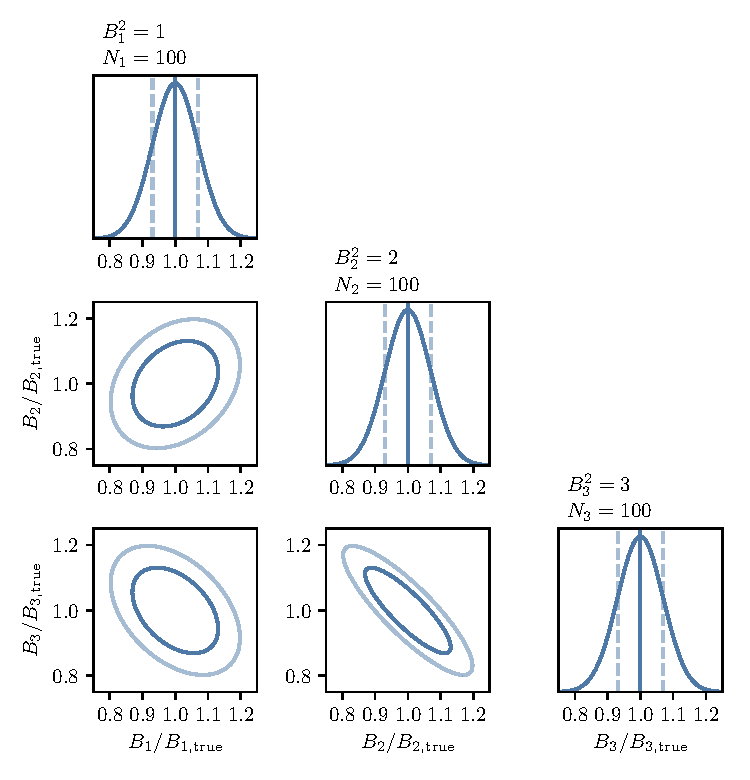
\includegraphics{fig/corner_Nconstant.pdf}
\end{center}
\caption{A toy corner plot showing the degeneracies between different lines
with different intrinsic \SN{} ratios under the white-noise dominated
assumption. We set $B_1^2 = 1$, $B_2^2 = 2$, and $B_3^2 = 3$ along with $N_1,
N_2, N_3 = 100$ and $V_k^2 = 2\times10^6$. Since each line has the same value
of $N$, the \SN{} of each line is driven by the value of $B_i$, with $B_3$
having the highest intrinsic \SN{} and $B_1$ the lowest. We plot each axis as
a fraction of the true value for each of $B_1$, $B_2$, and $B_3$, and see that
the marginalized posterior on each bias factor is the same (\textit{diagonal
panels}) as we expect from Equation~\ref{eq:frac_error_same}. There is a
strong negative covariance between $B_2$ and $B_3$, a mildly negative
covariance between $B_3$ and $B_1$, and a mildly positive covariance between
$B_1$ and $B_2$. An explanation for this behavior is given in the text.}
\label{fig:tf_Nconst}
\end{figure}

\begin{figure}[h!]
\begin{center}
\includegraphics{fig/corner_Nconstant_Bhigher.pdf}
\end{center}
\caption{We perform the same procedure as in Figure~\ref{fig:tf_Nconst}, except
now we slightly increase the intrinsic \SN{} of $B_2$ and $B_3$ by setting
$B_2^2 = 4$ and $B_3^2 = 9$. The values for each $N_i$ and $V_k$ are the same
as in Figure~\ref{fig:tf_Nconst}. We see that even though nothing about line
$1$ has changed (i.e. no additional measurements of line $1$ have been made),
the \SN{} on $B_1$ has improved because the fractional error on each line must
be the same (Equation~\ref{eq:frac_error_same}). The degeneracies between the
different lines discussed in Figure~\ref{fig:tf_Nconst} become stronger in
this case.}
\label{fig:tf_Nconst_Bhigher}
\end{figure}

Now we wish to consider how the \SN{} on each $B_i$ from the various
cross-spectra is related to the \SN{} in the auto-spectrum case. We first
write down the \SN{} from the auto-spectrum in the white-noise dominated
regime:
\beq \label{eq:autops_sn_wn}
\SN(B_1, \text{auto-spectrum}) = \frac{B_1^2}{N_1} V_k
\eeq

Now, let us compare the \SN{} of the two approaches in various cases. This
will be simpler to write if we introduce $\tilde{B}_i \equiv B_i^2/N_i$. Then,
\beq
\frac{\SN(B_1, \text{three-field})}{\SN(B_1, \text{auto-spectrum})} =
\frac{2}{\tilde{B}_1}
\sqrt{\frac{\tilde{B}_1\tilde{B}_2\tilde{B}_3}{\tilde{B}_1 + \tilde{B}_2 + \tilde{B}_3}}
\text{.}
\eeq
There are several interesting cases to consider with this formula. For
starters, let us assume that each field is measured to the same precision,
i.e. $\tilde{B}_1 = \tilde{B}_2 = \tilde{B}_3 = \tilde{B}$. In this case, we
have that
\beq
\frac{\SN(B_1, \text{three-field})}{\SN(B_1, \text{auto-spectrum})} =
\frac{2}{\sqrt{3}} \approx 1.15
\text{.}
\eeq
So, the three-field approach gives a marginally better \SN{} than the
auto-spectrum approach. This is encouraging, because it means that a tentative
auto-spectrum measurement could be checked against the value derived from the
three-field approach. Next, let us assume that the field $1$ has a much
stronger signal strength than $2$ or $3$ --- i.e. $\tilde{B}_1 \gg
\tilde{B}_2,\tilde{B}_3$. In this case we have that
\beq
\frac{\SN(B_1, \text{three-field})}{\SN(B_1, \text{auto-spectrum})} =
2\frac{\sqrt{\tilde{B}_2\tilde{B}_3}}{\tilde{B}_1}\text{.}
\eeq
In this case we see that it is unlikely for the $\text{S}/\text{N}$ on $B_1$
to be higher in the three-field case than in the auto-spectrum case. On the
other hand, let us consider the case where one of the other lines is measured
to much higher precision, e.g. $\tilde{B}_2 \gg \tilde{B}_1,\tilde{B}_3$. In
this case, we have that
\beq
\frac{\SN(B_1, \text{three-field})}{\SN(B_1, \text{auto-spectrum})} =
2\sqrt{\frac{\tilde{B}_3}{\tilde{B}_1}}\text{.}
\eeq
As long as field $1$ and $3$ are measured to comparable precision, a gain in
the \SN{} of $\sim2$ is possible with the three-field approach. Finally, let
us consider the most interesting case in which fields $2$ and $3$ are measured
to much higher precision than field $1$ --- i.e. $\tilde{B}_2, \tilde{B}_3 \gg
\tilde{B}_1$. For simplicity let us also assume that $\tilde{B}_2 \approx
\tilde{B}_3 = \tilde{B}$. In this case, we have that
\beq
\frac{\SN(B_1, \text{three-field})}{\SN(B_1, \text{auto-spectrum})} =
\sqrt{2}\sqrt{\frac{\tilde{B}}{\tilde{B}_1}}
\text{.}
\eeq
As a result, if two lines are measured with strong precision, then we can
strongly boost the \SN{} of a third, weakly measured line with the three-field
approach.

As an illustration, we construct a corner plot in Figure~\ref{fig:tf_Nconst}
for the inferred bias values using toy values of $B_1^2 = 1$, $B_2^2 = 2$, and
$B_3^2 = 3$ along with $N_1, N_2, N_3 = 100$ and $V_k^2 = 2\times10^6$. The
units here are arbitrary. Since each line has the same value of $N$, the \SN{}
of each line is driven by the value of $B_i$, with $B_3$ having the highest
intrinsic \SN{} and $B_1$ the lowest. We make the same assumptions that go
into Equation~\ref{eq:fmat_tf_exp}, i.e. that we are white-noise dominated in
each line. By plotting each axis as a fraction of the true value for each of
$B_1$, $B_2$, and $B_3$, we see that the marginalized posterior on each bias
factor is the same (\textit{diagonal panels}). This is equivalent to saying
that the fractional error on each bias factor is the same for each line.

Moving on to the joint panels in Figure~\ref{fig:tf_Nconst}, we see that there
is a strong negative covariance between $B_2$ and $B_3$, a mildly negative
covariance between $B_3$ and $B_1$, and a mildly positive covariance between
$B_1$ and $B_2$. We can intuitively understand this behavior by considering
that each cross-spectrum places a prior on the product $B_1B_2$, $B_2B_3$, and
$B_3B_1$, with the width of that prior given by the \SN{} of that
cross-spectrum.

In this toy scenario, the product $B_2B_3$ will have the highest \SN{} and
therefore the tightest prior, and therefore to account for a larger $B_3$ one
must have a smaller $B_2$ (and vice-versa), hence the strong negative
correlation. We can make this argument for the relationship between $B_2$ and
$B_3$ since $B_2B_3$ has the tightest prior, and therefore the products
$B_1B_2$ and $B_3B_1$ are not relevant, since they have wider priors. The next
tighest prior is on the product $B_3B_1$. Increasing the value of $B_1$ means
that we must decrease the value of $B_3$ to keep $B_3B_1$ constant. Since
$B_2B_3$ has a tighter prior, this means that we must also decrease the value
of $B_2$. The prior on $B_1B_2$ is irrelevant, since it is wider than the
other two.\footnote{Although in this case, to keep $B_1B_2$ constant while
increasing $B_1$ we would need to decrease $B_2$ anyways.}

Finally, we turn to the product $B_1B_2$, which has the widest prior of the
three products. If we increase $B_1$, then naively we would need to decrease
$B_2$. However, increasing $B_1$ also means that we must decrease $B_3$ to
keep $B_3B_1$ constant. Furthermore, decreasing $B_3$ means that we must
increase $B_2$ to keep $B_2B_3$ constant. Since the priors on $B_2B_3$ and
$B_3B_1$ are tighter than on $B_1B_2$, these constraints dominate, and as a
result increasing $B_1$ means that we must increase $B_2$. Therefore, $B_1$
and $B_2$ are positively correlated.

In Figure~\ref{fig:tf_Nconst_Bhigher} we perform the same procedure, except
now we slightly increase the intrinsic \SN{} of $B_2$ and $B_3$ by setting
$B_2^2 = 4$ and $B_3^2 = 9$. Notice that we have not changed the intrinsic
\SN{} of field $1$. Two things are apparent. First, the strength of the
correlations that we discussed for Figure~\ref{fig:tf_Nconst} are stronger,
since the different priors have become more disparate in their relative
tightness. Second, as a consequence of the fractional \SN{} being the same for
each line, we see that the error on $B_1$ has become much smaller (and
similarly for $B_2$ and $B_3$). However, this is particularly interesting in
the case of $B_1$. No modification has been made to it's intrinsic \SN{} (or,
in other words, no additional measurements have been made of line $1$).
Nonetheless, the \SN{} on the inferred $B_1$ has become higher.

\subsection{Interloping Lines} \label{ssec:interlopers}
The multi-field method relies only on the measurements of cross-spectra beween
various lines. Interloping lines do not contribute to the average
cross-spectra signal, but does contribute to the noise of the measurement. We
can account for this by modifying the equation for $N_i$ to be
\citep{2016ApJ...825..143L, 2016ApJ...832..165C},
\beq\label{eq:ptot_intlpr}
N_i = N_{i,\text{instrumental}} + \sum_{j} \frac{1}{\apar(z_j) \aperp(z_j)^2} 
            P_j\left(\frac{\kpar}{\apar(z_j)}, 
                     \frac{\kperp}{\aperp(z_j)}\right)\text{,}
\eeq
where $N_{i,\text{instrumental}}$ is the instrumental noise of line $i$ at the
observed frequency, the sum on $j$ is over all interloping lines, $z_j$ is the
emitted redshift of line $j$, and where,
\begin{alignat}{2}
\apar = \frac{H(z_i)}{H(z_j)} \frac{1+z_j}{1+z_i} \quad \quad &&
\aperp = \frac{D_{A}(z_j)}{D_A(z_i)}\text{,}
\end{alignat}
where $z_i$ is the emitted redshift of line $i$ and $D_A(z)$ is the comoving
angular diameter distance to redshift $z$. For simplicity, we assume the
instrumental noise is white (i.e. $N_{i,\text{instrumental}}$ is constant),
though it is straightforward in this formalism to incorporate a $k$- or
$\mu$-dependence in the instrumental noise.

Unlike in the three field case, where the integrand of the Fisher matrix was
only dependent on $k$, the noise and therefore covariance matrix depends also
on $\mu$. Galactic foregrounds can imprint an azimuthal dependence as well,
which we do not consider in this work. Incorporating a polar dependence is straightforward, and we can write the Fisher matrix as:
\beq\label{eq:fisher_mu}
F_{i,j} = 
\int \frac{\text{d}k\,\text{d}\mu}{(2\pi)^2} k^2 V_{\text{surv}}
% \int \frac{\text{d}k\,k^2}{2\pi^2} V_{\text{surv}} 
\sum_{l} \sum_{m}
\frac{\partial \hat{P}_{l}(k, \mu)}{\partial B_i}
\left(\Cov{\hat{P}_{l}(k, \mu)}{\hat{P}_{m}(k, \mu)}\right)^{-1}
\frac{\partial \hat{P}_{m}(k, \mu)}{\partial B_j}\text{,}
\eeq



% \begin{multicols}{2}
%   \beq
%     \apar = \frac{H(z_i)}{H(z_j)} \frac{1+z_j}{1+z_i}
%   \eeq\break
%   \beq
%     \aperp = \frac{D_{A}(z_j)}{D_A(z_i)}
%   \eeq
% \end{multicols}

% \begin{figure}[h!]
% \begin{center}
% 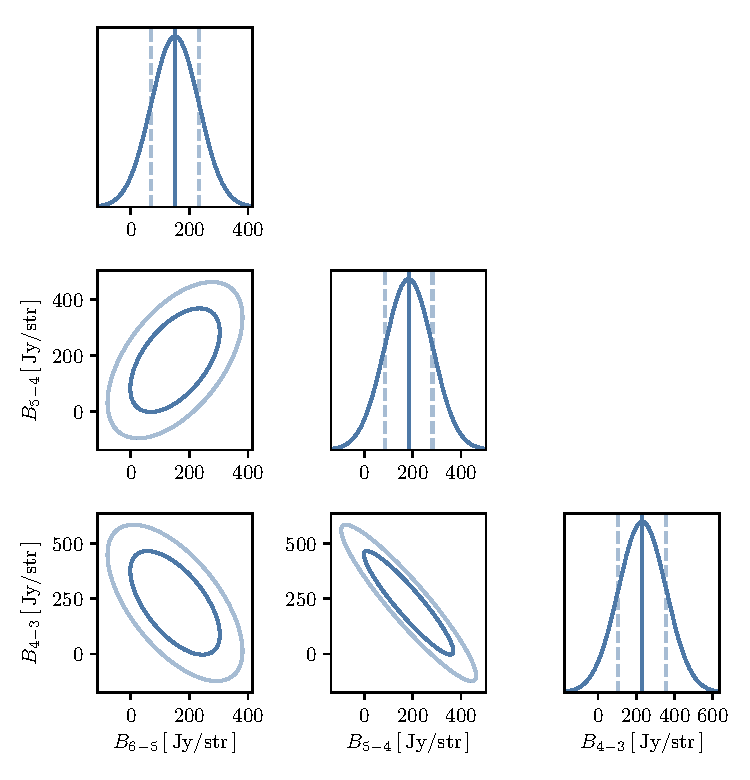
\includegraphics{fig/CO_tf.pdf}
% \end{center}
% \caption{Constraints that can be placed on the fluctuations of the \CO(6-5),
% \CO(5-4), and \CO(4-3) lines with CCAT-p at $z_{\text{obs}} = 0.88$. This
% Figure is purely illustrative, as we do not include noise contributions from
% residual foreground contamination or interloper/extraloper lines. According to
% our simple \CO{} model, we have that $B_{\text{6-5}}, B_{\text{5-4}},
% B_{\text{4-3}} = 151, 183, 232\,\text{Jy}/\text{str}$. Using the instrumental
% specifications in \citet{2018arXiv181208135C}, we find that $N_{\text{6-5}},
% N_{\text{5-4}}, N_{\text{4-3}} = 5.1\times10^9, 1.4\times10^9,
% 5.4\times10^8\,\left(\text{Jy}/\text{str}\right)^2\,\Mpc^3$. We find the same
% behavior as in Figure~\ref{fig:tf_Nconst}, where the best-measured line is
% strongly negatively degenerate with the second-best measured line, the
% best-measured and worst-measured are slightly negatively degenerate, and the
% second-best measured line and the worst-measured are slightly positively
% degenerate. }
% \label{fig:CO_tf}
% \end{figure}

% Armed with some intuition from the simple white noise-dominated case, we now
% turn to forecasting constraints that can be placed on the \CO{} bias factors.
% Our modelling of the \CO{} intensity as a function of redshift follows
% \citet{2016ApJ...825..143L} and is outlined in Appendix~\ref{app:co_int}. We
% assume that $b_i=3$ for each \CO{} line.

% At $z=0.88$, the lines \CO(6-5) ($\nu_{\text{obs}} = 367\,\MHz$), \CO(5-4)
% ($\nu_{\text{obs}} = 306\,\MHz$), and \CO(4-3) ($\nu_{\text{obs}} =
% 245\,\MHz$) are all in the observing band of CCAT-p. We only include
% instrumental noise for this Subsection, neglecting foreground and
% interloper/extraloper contamination. We simply want to place the result of
% Section~\ref{ssec:tf_noisedom} in the context of an actual experiment.

% Using our \CO{} modelling, we find that $B_{\text{6-5}}, B_{\text{5-4}},
% B_{\text{4-3}} = 151, 183, 232\,\text{Jy}/\text{str}$ at $z=0.88$. Using the
% instrumental specifications in \citet{2018arXiv181208135C}, we find that
% $N_{\text{6-5}}, N_{\text{5-4}}, N_{\text{4-3}} = 5.1\times10^9,
% 1.4\times10^9, 5.4\times10^8\,\left(\text{Jy}/\text{str}\right)^2\,\Mpc^3$. We
% assume the instrumental noise is white, but note that in this case the
% noise-dominated assumption is mildly broken. The worst case is that of the
% \CO(4-3) line, where on a scale of $k\sim0.01\,\Mpc^{-1}$ we have that
% $P_{\text{4-3}} \sim 3N_{\text{4-3}}$. Again, this Subsection is purely
% illustrative, and we will rectify these assumptions in the next Section.

% We assume a bandwidth of $60\,\MHz$ for the line \CO(6-5). This corresponds to
% a redshift band of width $\Delta z = 0.16$. We resize the \CO(5-4) and
% \CO(4-3) bands to have the same extent in redshift space, which means slightly
% scaling the frequency bandwidth --- in this case, the bandwidths are $50$ and
% $40\,\MHz$, respectively. In Figure~\ref{fig:CO_tf} we show the constraints
% that can be placed on each of $B_{\text{6-5}}$, $B_{\text{5-4}}$, and
% $B_{\text{4-3}}$. The line \CO(4-3) is measured to the best intrinsic \SN{},
% followed by \CO(5-4) and then \CO(6-5). We find the same behavior as in
% Section~\ref{ssec:tf_noisedom}, where the best-measured line is strongly
% negatively degenerate with the second-best measured line, the best-measured
% and worst-measured are slightly negatively degenerate, and the second-best
% measured line and the worst-measured are slightly positively degenerate.
% However, we find that CCAT-p should be able to make a measurement of each bias
% factor using the three-field approach.

\section{Random Thoughts}
Like doing a matched filter??? Trying to understand intuitively why this
works. If you have a super well measured field, then its like you're God who
knows that the density field is. Its almost like using that density field as a
matched filter?

\appendix
\section{CO Intensity Modelling} \label{app:co_int}
To model the statistical fluctuation and amplitude of the \CO{} intensity maps
we follow \citet{2016ApJ...825..143L}, and briefly summarize the procedure
here. We begin by assuming a Schechter form for the star formation rate
function,
\beq\label{eq:schechter}
\phi(\SFR)\,\text{d}\SFR = \phi_*
\left(\frac{\SFR}{\SFR_*}\right)^{\alpha}\exp{\left[-\frac{\SFR}{\SFR_*}\right]}
\frac{\text{d}\SFR}{\SFR_*}
\eeq
where $\alpha$ is the faint-end slope, $\SFR_*$ is the characteristic
star-formation rate, and $\phi_*$ is the characteristic number density. The
average specific intensity in a line $l$ can be related to the comoving
emissivity by \citep{2011ApJ...741...70L, 2013ApJ...768...15P},
\beq\label{eq:emiss_to_int}
\avg{I_l} = \frac{\epsilon_l}{4\pi \nu_{\text{rest},l}}\frac{c}{H(z)}\text{,}
\eeq
where $\nu_{\text{rest},l}$ is the rest-frame emission frequency and
$\epsilon_l$ is the comoving emissivity, each of line $l$. Assuming a linear
luminosity-SFR relation with a constant of proportionality of $L_0^l$, along
with the Schechter form for the SFR function (Equation~\ref{eq:schechter}), it
follows that \citep{2013ApJ...768...15P},
\beq\label{eq:com_emiss}
\epsilon_l = \phi_* L_0^{l}
\frac{\SFR_*}{1\,\Msun\text{yr}^{-1}}\Gamma{(2+\alpha)}\text{.}
\eeq
We adopt the value of $L_0^{\CO}$ for each line transition from
\citet{2010JCAP...11..016V}.


\bibliography{references}

\end{document}
